\documentclass[a4paper,10pt,openany,oneside]{report}

% - PACKAGES -
\usepackage[left=2.5cm,right=2.5cm,top=3cm,bottom=3cm,headsep=1cm]{geometry}
\usepackage{graphicx}
\usepackage{tabularx}
\usepackage{amsfonts}
\usepackage{pstricks}
\usepackage{amsmath}
\usepackage{amssymb}
\usepackage[french]{babel} 
\usepackage{changepage}
\usepackage{color}
\usepackage{enumitem}
\usepackage{fancyhdr}
\usepackage[T1]{fontenc}
\usepackage[utf8]{inputenc}
\usepackage[hidelinks]{hyperref}
\usepackage{listings} %Pour le code
\usepackage{titlepic}
\usepackage{wrapfig}
\usepackage{longtable}
\usepackage{hyperref}
\usepackage{enumitem}
\usepackage{titlesec}
\usepackage{python}
\usepackage[11pt]{moresize}
\usepackage{fancyhdr}
\usepackage{lastpage}

% - COLORS -
\definecolor{myblue}{rgb}{0,0,1}
\definecolor{mylightgray}{rgb}{0.9,0.9,0.9}
\definecolor{dkgreen}{rgb}{0,0.6,0}
\definecolor{mauve}{rgb}{0.58,0,0.82}

% - OTHER SETTINGS -
\lstset{language=Python,
  frame=tb,
  label={lst:code_direct},
  basicstyle=\footnotesize,
  keywordstyle=\color{blue},
  aboveskip=3mm,
  belowskip=3mm,
  showstringspaces=false,
  columns=flexible,
  basicstyle={\small\ttfamily},
  numbers=left,
  numberstyle=\normalsize,
  numbersep=7pt,
  numberstyle=\tiny\color{black},
  keywordstyle=\color{blue},
  commentstyle=\color{dkgreen},
  stringstyle=\color{mauve},
  breaklines=true,
  breakatwhitespace=true,
  tabsize=4
}
\pagestyle{fancy}

% - DOCUMENT -
\begin{document}

% - FRONT PAGE -
\thispagestyle{empty}
\vspace*{0.5cm}
\setlength{\parindent}{0cm}
\pagenumbering{arabic}

\begin{center}
\textbf{\Large Rapport de Traitement d'Image}\\
\vspace*{3cm}
\textbf{\Huge Détection de panneau de signalisation}\\[3cm]
Ce rapport a pour but de décrire les différentes étapes et technologies explorer lors de notre projet de traitement d'image
\vspace*{3cm}

\large{Réalisé par\\
 \Large{Damian \bsc{Petroff}\\
 Segan \bsc{Salomon}}}\\[0.3cm]
\large{Supervisé par François \bsc{Tièche}}\\[5cm]
\begin{figure}[!h]
\centering

\includegraphics[width=0.2\textwidth]{../img/hearc.jpg}
\end{figure}
\textit{\today}\\[3cm]
\end{center}

\pagebreak


\titleformat{\chapter}[display]
{\normalfont\huge\bfseries}{\chaptertitlename\ \thechapter}{20pt}{\Huge}   
\titlespacing*{\chapter}{0pt}{-50pt}{40pt}
\setitemize{topsep=5pt}
\setlength{\parindent}{1em}

% - TABLE OF CONTENTS -
\tableofcontents
\thispagestyle{empty}
\pagebreak
\setcounter{page}{1}

% - BODY -

\chapter{Introduction}


\chapter{Expérimentation}

Dans ce chapitre seront répertoriées les diverses expérimentations ayant conduits au résultat final de Panno.

\section{Partie IA (Tri entre "image avec panneau" et "image sans panno")}
Pour la première partie du projet, qui est de filtrer et garder uniquement les images contenant des panneaux, le but a été d'entraîner un modèle avec pleins d'images contenant des panneaux et d'autre ne contenant pas de panneau.

\subsection{Problème de l’acquisition d'images d'entraînement / test}
Un des premiers problèmes a été de trouver des images, plusieurs solutions existantes :
\begin{enumerate}
\item Prendre des images nous-même, cette façon de faire est très coûteuse en temps mais pourrait permettre d'avoir les meilleures images pour l'apprentissage car les images de tests doivent être prise depuis l'habitacle d'une voiture, ainsi prendre des images d'entraînement nous-même depuis l'habitacle d'une voiture justement.
\item Chercher des images existantes sur internet. Le problème que l'on remarque immédiatement est déjà qu'un dataset d'image de la même nature que celle dont on a besoin est relativement introuvable, ou alors ne correspond pas aux genre de panneau de signalisation que nous recherchons. Nous avons trouvé certains dataset et entraîné, mais ils ne fournissent pas de bons résultats dû à la nature complètement différente de notre problème. En effet la plupart des datasets ont pour objectif de classifier par panneau (multi-classes) alors que nous cherchons à classifier entre "panneau" et "pas panneau" ce qui est un problème de classification binaire.
\item Prendre des captures d'écran de Google Street View. Cette dernière option semble être la plus faisable en terme de temps / efficacité. Nous avons donc décider de prendre quelques images venant de cette source pour entraîner notre modèle.
\end{enumerate}

\subsection{Problème de la quantité d'images}
En effet il est impossible d'obtenir de bons résultats avec un jeu de données d'uniquement des dizaines d'images, il en faudrait au moins quelques milliers pour chacune des deux classes. Pour avoir une telle quantité d'images il faudrait passer des heures à prendre des captures d'écran de Google Street View, ce qui n'est absolument pas possible en terme de temps.

La solution directe à ce problème est donc d'augmenter ce jeu d'images en utilisant des fonctions d'OpenCV. C'est à ce moment là que nous nous sommes rendu compte qu'OpenCV lui-seul pouvait nous permettre de classifier ces images.

\subsection{Remplacement de la partie IA par un meilleur algorithme via OpenCV}
Lors de l'augmentation d'images, nous avons cherché à générer de nouvelles images ayant du sens, c'est-à-dire que plutôt d'ajouter du bruit inutile, nous cherchions à filtrer l'image de manière à l a rendre plus représentative et dans l'idéal faire ressortir un potentiel panneau de signalisation.\\

Pour ce faire, nous avons privilégié les canaux de couleur rouge et bleus, qui sont les couleurs principales des panneaux de signalisation, le vert n'étant présent que sur les panneaux d'autoroute.\\

En faisant un tel filtrage, nous nous somme rendu compte que le recherche de cercle avec la méthode de Hough permet de détecter les panneaux lorsqu'il y en a, et ne détecte aucun cercle sur une images où il n'en a pas, ce qui résout le problème de classification.

\subsection{Algorithme}
\subsubsection{Coupage de la composante verte}
La première étape est de couper le canal vert. Pour ce faire, on itère sur chaque pixel de l'image, et si sa composante verte est plus grande que les deux autres, on mets les trois composantes du pixel au même niveau qui est le maximum des trois composante, ceci remplace ce pixel majoritairement vert par un pixel gris. Cette algorithme est implémenté par la fonction $cut_green(img, criteria="max")$ le critère peut être réglé entre $max$, $min$ et $average$, ce dernier critère remplace les composantes du pixel par la moyenne des trois composantes.\\

Le résultat est le suivant :
\begin{figure}[!h]
\centering
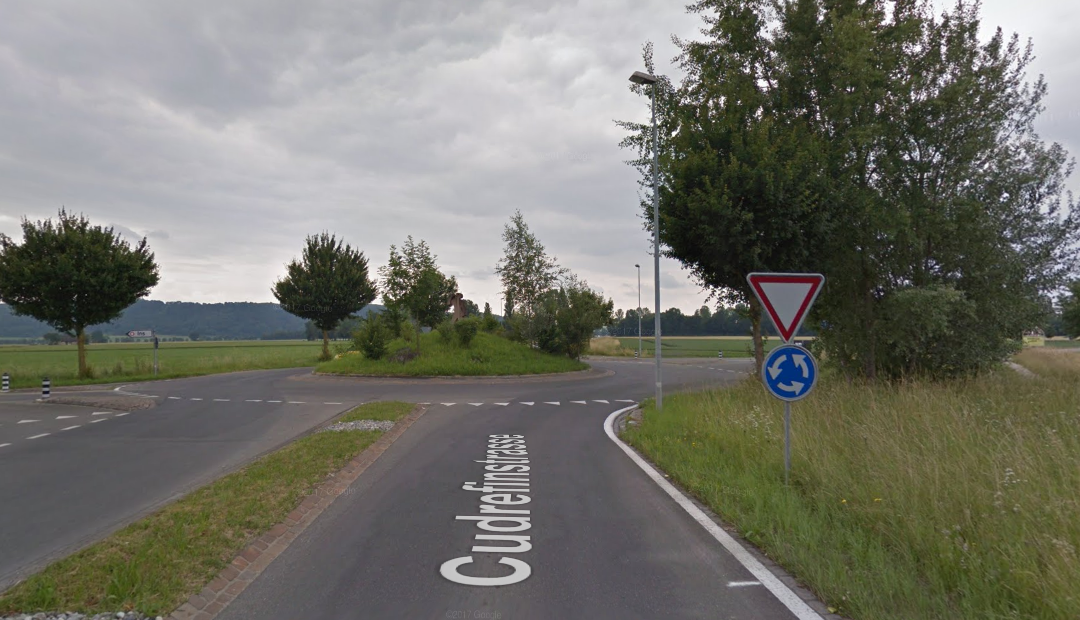
\includegraphics[width=0.7\textwidth]{../img/80-original.png}
\caption{Image originale}
\end{figure}

\begin{figure}[!h]
\centering
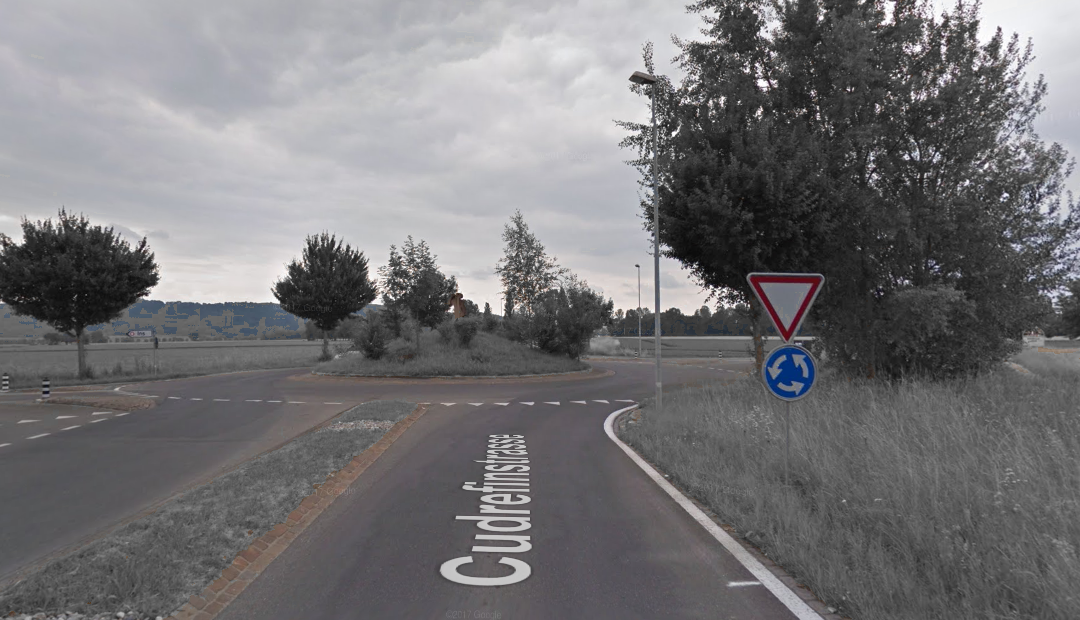
\includegraphics[width=0.7\textwidth]{../img/81-cut.png}
\caption{Image avec vert coupé}
\end{figure}

\subsubsection{Filtre réduisant le bruit sur l'image}
Ici le but a été de réduire le bruit dans l'image sans réduire la netteté du panneau. Le meilleur filtre que nous avons trouvé pour faire une telle chose est la fonction bilateralFilter d'OpenCV à laquelle nous avons donnné les paramètre suivants :
\[ cv2.bilateralFilter(img,30,50,50) \]
car ce sont ceux qui donnent les meilleurs résultats, que voici :

\begin{figure}[!h]
\centering
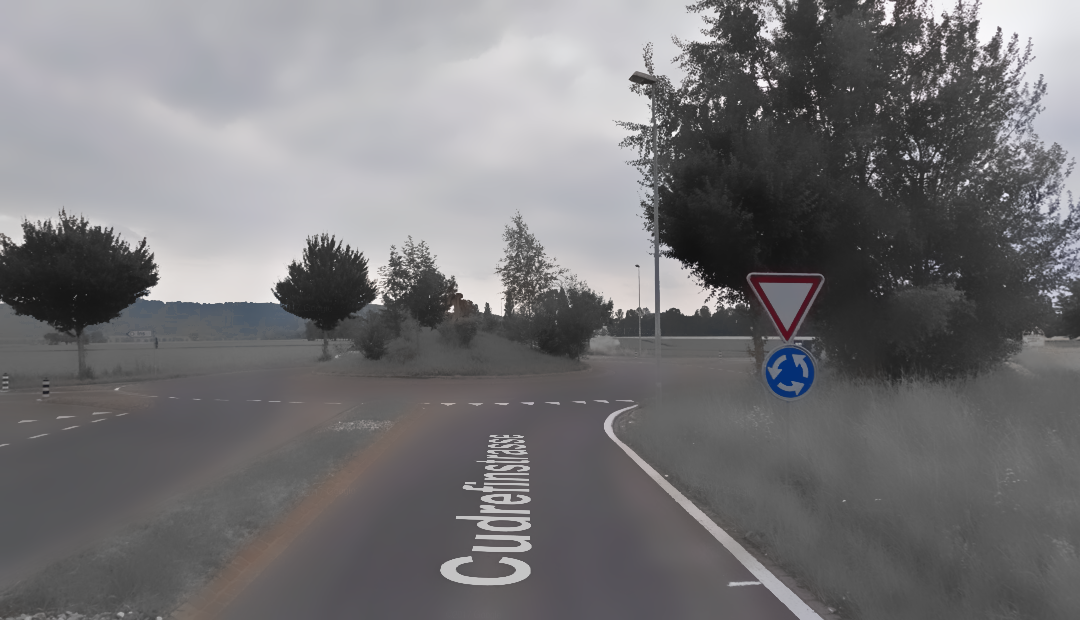
\includegraphics[width=0.7\textwidth]{../img/82-bilblur.png}
\caption{Image avec vert coupé et filtre bilatéral}
\end{figure}

On observe clairement que certains détails de l'image ce sont estompés, cela se remarque particulièrement dans les nuages et l'herbe. On voit également que les panneaux restent parfaitement net.

\subsubsection{Séparation et seuillage des composantes bleue et rouges}
La suite de l'algorithme consiste à séparer les composante bleue et rouge à les seuiller, puis à les additionner afin d'obtenir le résultat suivant :

\begin{figure}[!h]
\centering

\includegraphics[width=0.7\textwidth]{../img/84-redblue.png}
\caption{Image avec vert coupé et filtre bilatéral}
\end{figure}

\subsubsection{Suite de l'algorithme}
La suite de l'algorithme est celle déjà présente dans la partie détection du panneau.


\section{Partie détection (Recherche du panneau dans une image classifiée prétraitée}
\subsection{Fonctionnement}
Une fois l'image prétraitée celle-ci est passée au travers de 3 analyseurs pour découper les régions possédant probablement un panneau.
\begin{itemsize}
\item[-] Cercles de Hough
\item[-] Lignes probabilistiques de Hough
\item[-] Détection de contour
\end{itemsize}
La recherche des cercles permet de détecter les panneaux ronds, cette méthode est relativement fiable et permet de détecter, dans la plupart des cas un panneau dans divers environnements.
\begin{figure}[!h]
\centering
\includegraphics[width=0.7\textwidth]{../img/11-hough_circles.png}
\caption{Détection du panneau de limitation de vitesse}
\end{figure}

La deuxième méthode donnant les meilleurs est la détection de contour fourni par OpenCV.
\begin{figure}[!h]
\centering
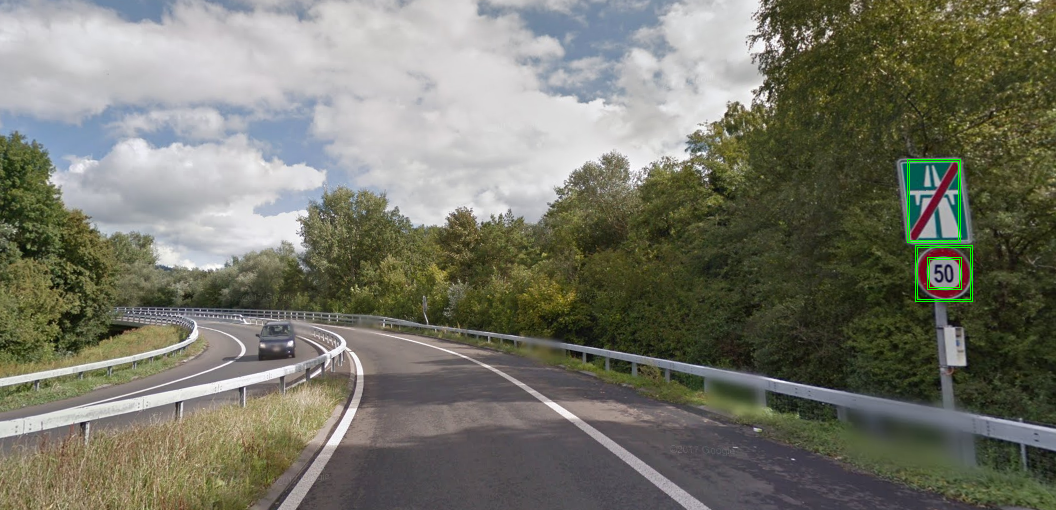
\includegraphics[width=0.7\textwidth]{../img/10-contour.png}
\caption{Détection des panneauxl}
\end{figure}

Pour chaque cercle ou région détectée, la zone est découpée dans l'image original et exportée dans un dossier.
\begin{figure}[!h]
\centering
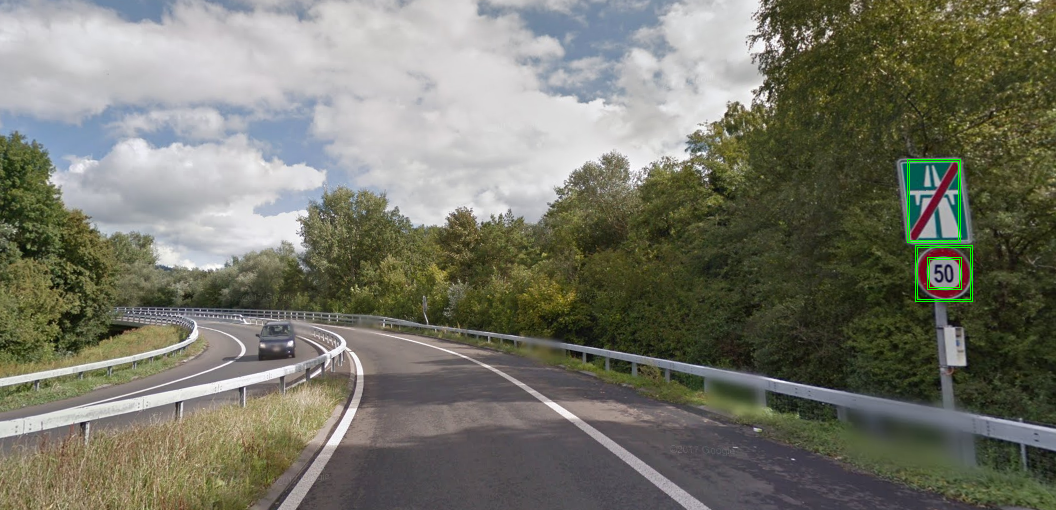
\includegraphics[width=0.7\textwidth]{../img/10-contour.png}
\caption{Extraction du panneau}
\end{figure}

\subsection{Etapes de recherches}
\subsubsection{Première itération}
Développement de l'algorithme de base. 
\begin{itemize}
\item[-] Normalisation de l'image
\item[-] Canny
\item[-] Ouverture avec un kernel de (5, 5)
\item[-] Gradient avec le même kernel
\end{itemize}

\subsubsection{Deuxième itération}
\begin{itemize}
\item[-] Ajout d'un filtre median avant la normalisation
\item[-] Réduction de la taille du kernel à (3, 3)
\item[-] Ajout de la dilatation
\item[-] Ouverture
\item[-] Canny
\item[-] Fermeture
\end{itemize}

\subsubsection{Troisième itération (Ajout de Hough)}
\begin{itemize}
\item[-] Ajout de Hough pour détecter les contours
\item[-] Essaies avec diverses valeurs pour trouver les meilleures paramètres
\item[-] Utilisation d'une image de qualité (4k original)
\end{itemize}

\subsubsection{Ajout du crop}
\begin{itemize}
\item[-] Ajout du découpage des régions intéressantes (Cercles uniquement dans un premier temps)
\item[-] Remplacement du filtre médian par un filtre gaussien pour de meilleurs résultats
\item[-] Ajout d'une méthode pour enregistrer les images
\end{itemize}

\subsubsection{Ajout de la détection de contour}
\begin{itemize}
\item[-] Ajout des méthodes OpenCV permettant de découper des régions détourées depuis les images prétraitées
\item[-] Mise en place d'une structure de dossier pour la sortie des analyses
\end{itemize}

\chapter{Résultats}
Les résultats sur les images testées sont plutôt convainquant, tous les panneaux ronds et isolés sont détectés par la méthode de Hough s'ils ont une taille suffisamment grande.
Les panneaux rectangulaires et mêmes ronds sont également relativement biens détectés par la méthode de détection de contour d'OpenCV avec les images prétraitées.

\section{Cercle de Hough}
\begin{figure}[!h]
\centering
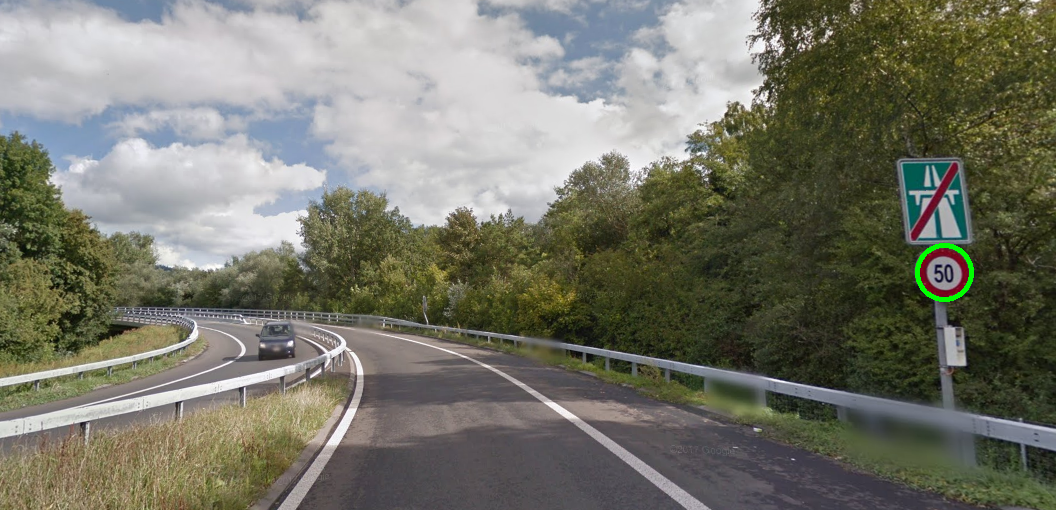
\includegraphics[width=\textwidth]{../img/19-hough_circles.png}
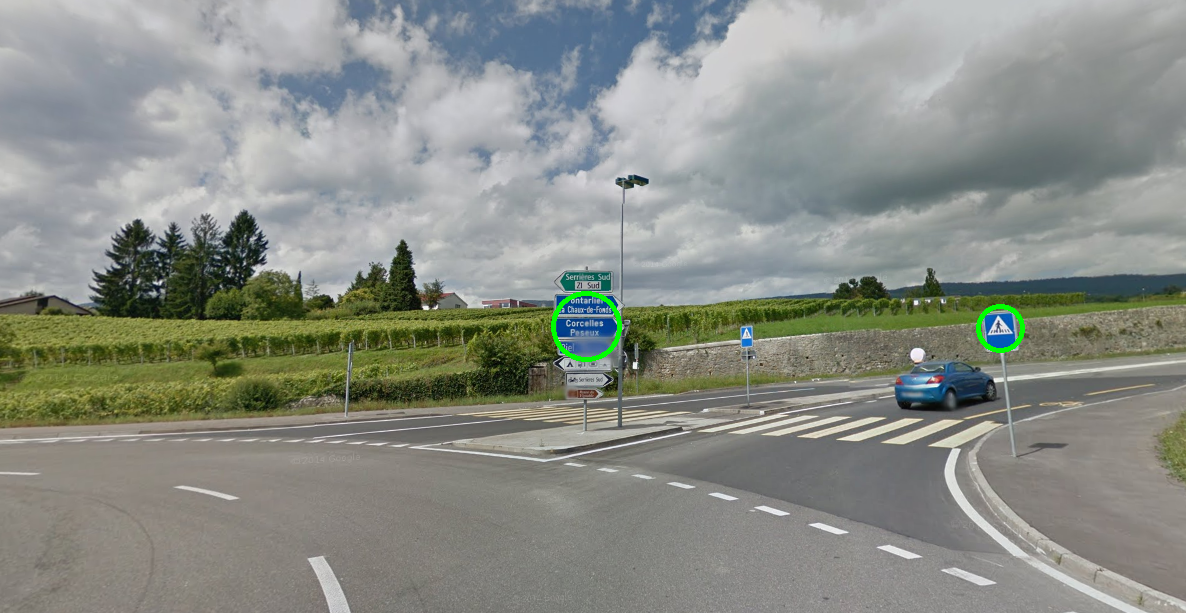
\includegraphics[width=\textwidth]{../img/39-hough_circles.png}
\end{figure}
\pagebreak

\begin{figure}[!h]
\centering
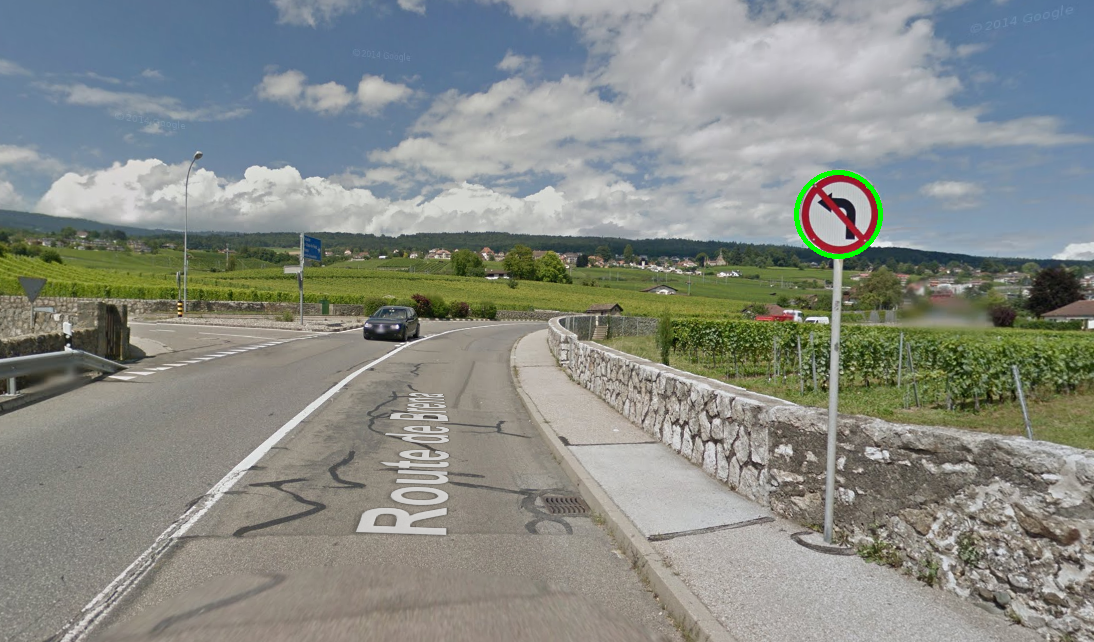
\includegraphics[width=0.8\textwidth]{../img/49-hough_circles.png}
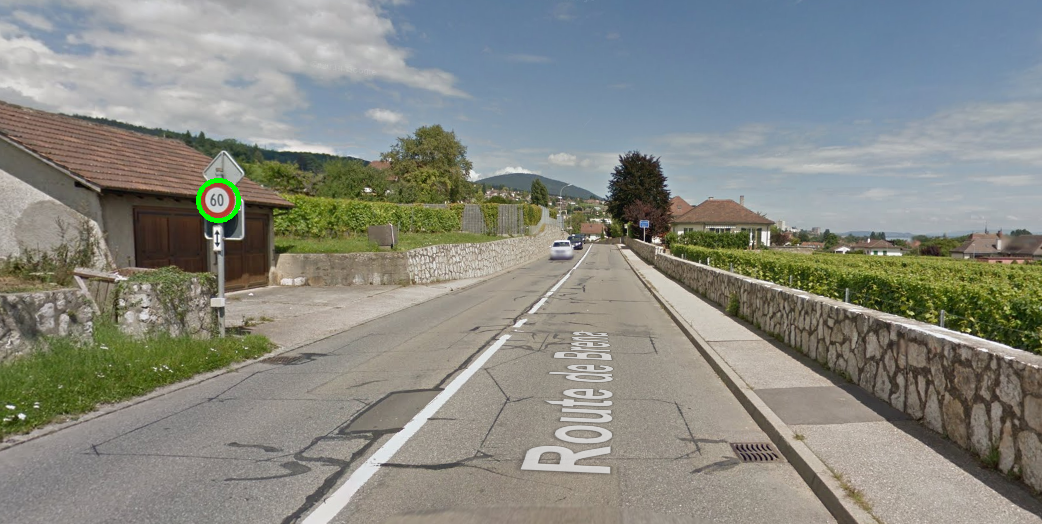
\includegraphics[width=0.8\textwidth]{../img/59-hough_circles.png}
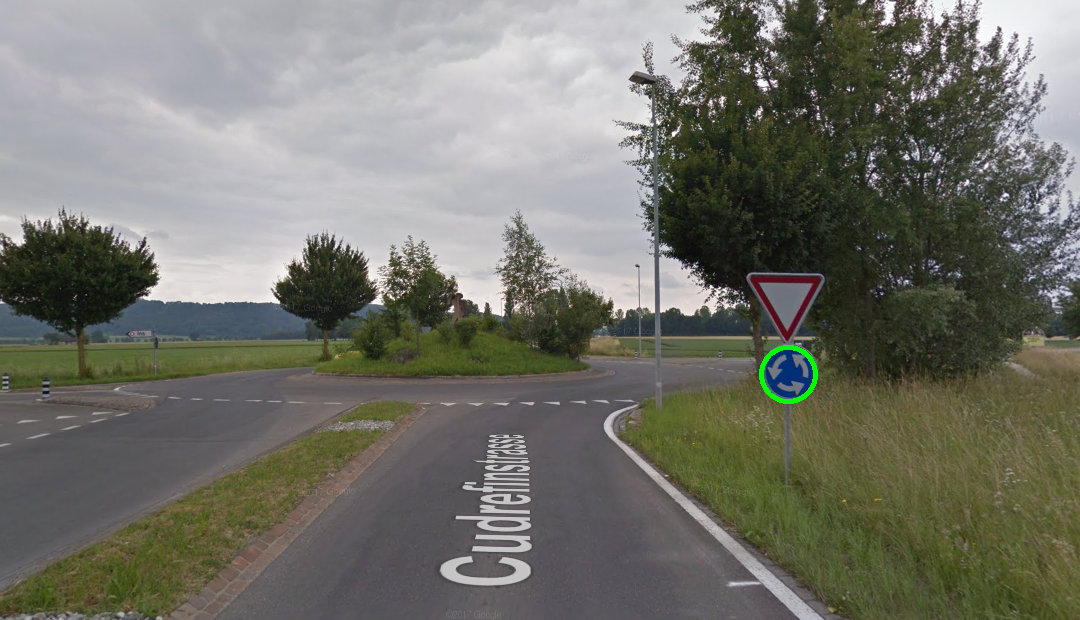
\includegraphics[width=0.8\textwidth]{../img/89-hough_circles.png}
\end{figure}
\pagebreak

\section{Lignes de Hough}


\section{Bugs}
\subsection{Panneaux circulaires}
Certaines images où les panneaux sont trop sombres ne sont pas très bien seuillées et des problèmes de détection de cercle apparaissent. Soit trop de cercles sont détectés, soit aucun cercle n'arrivent à être trouvé. Ce problème est particulièrement présent lorsque les panneaux sont sur-expositionné ou sous-expositionné, comme dans les cas de contre-jour ou d'ensoleillement direct, comme le montre les deux images suivantes :

\begin{figure}[!h]
\centering
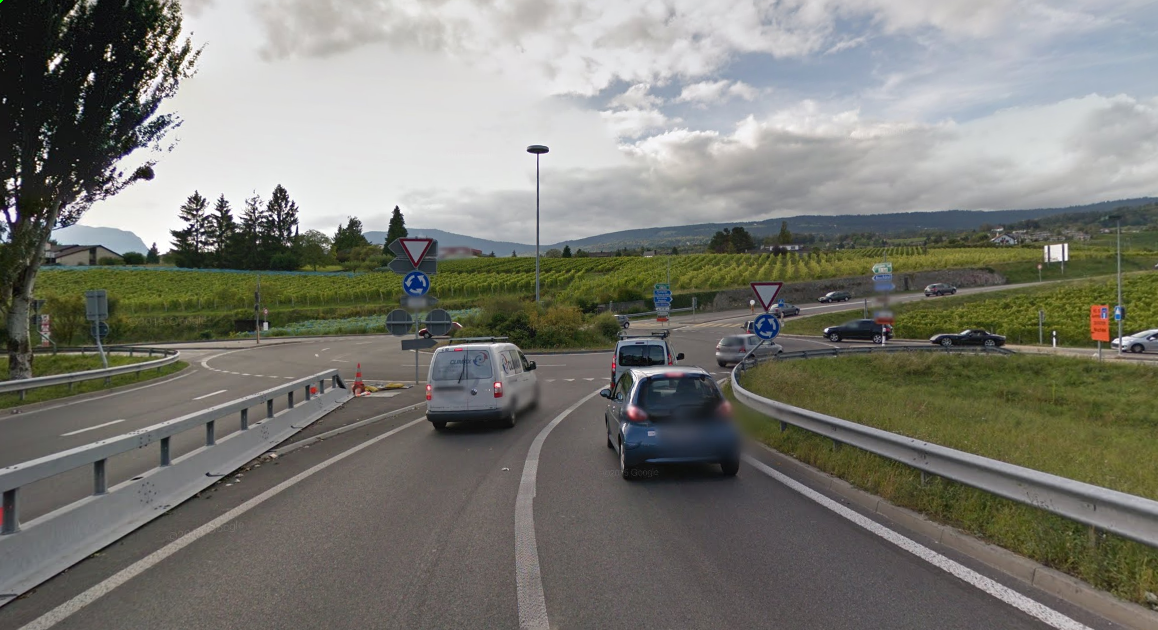
\includegraphics[width=\textwidth]{../img/29-hough_circles.png}
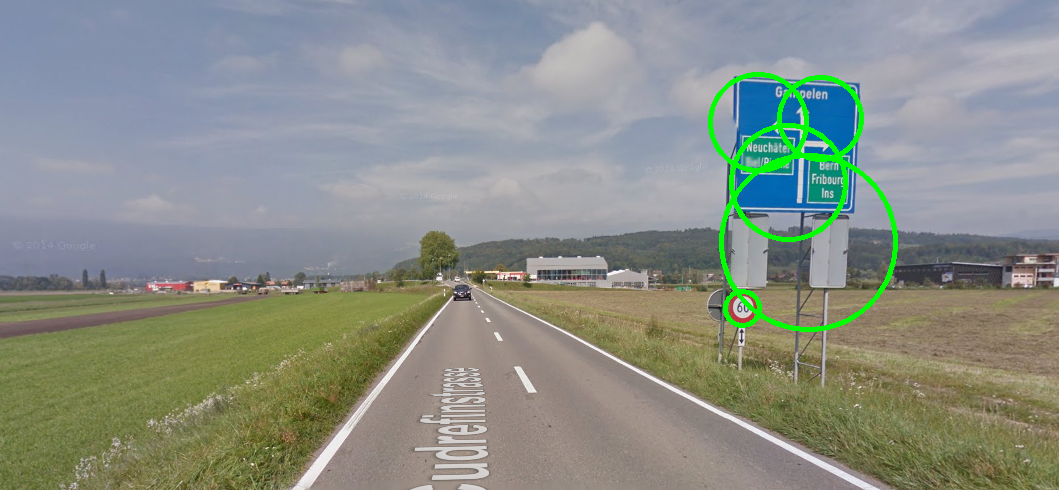
\includegraphics[width=\textwidth]{../img/69-hough_circles.png}
\end{figure}
\pagebreak
\subsection{Panneaux rectangulaires}


\chapter{Conclusion}

\end{document}


